\documentclass[11pt, oneside]{article}   	% use "amsart" instead of "article" for AMSLaTeX format

\usepackage{jmlr2e}
\usepackage{lineno}
\linenumbers
%\jmlrheading{1}{2014}{X-XX}{4/00}{10/00}{Kyle Cranmer}

%\ShortHeadings{Likelihood ratio tests constructed with discriminative classifiers and calibrated with generative models}{Kyle Cranmer}


\usepackage{geometry}                		% See geometry.pdf to learn the layout options. There are lots.
\geometry{letterpaper}                   		% ... or a4paper or a5paper or ... 
%\geometry{landscape}                		% Activate for for rotated page geometry
%\usepackage[parfill]{parskip}    		% Activate to begin paragraphs with an empty line rather than an indent
\usepackage{graphicx}				% Use pdf, png, jpg, or eps§ with pdflatex; use eps in DVI mode
								% TeX will automatically convert eps --> pdf in pdflatex		
\usepackage{amssymb, amsmath}
\usepackage{algorithm}
\usepackage{algorithmic}
\usepackage{xfrac}

\DeclareMathOperator*{\argmin}{arg\,min}
\DeclareMathOperator*{\argmax}{arg\,max}

%\title{Likelihood ratio tests constructed with discriminative classifiers and calibrated with generative models}
\title{Likelihood ratio tests constructed with discriminative classifiers and calibrated with generative models}
%\title{Calibrated, Parametrized Learning}
\author{Kyle Cranmer}
%\date{}							% Activate to display a given date or no date

\begin{document}


\author{\name Kyle Cranmer \email kyle.cranmer@nyu.edu \\
       \addr Center for Cosmology and Particle Physics\\
       Center for Data Science\\
       New York University \\
       New York, NY 10003, USA
}

%\editor{Leslie Pack Kaelbling}
\editor{}

\maketitle

\begin{abstract}%   <- trailing '%' for backward compatibility of .sty file
We demonstrate how discriminative classifiers can be used to approximate 
generalized likelihood ratio tests over high-dimensional data when a generative model 
for the data is available for training and calibration.  
\end{abstract}
%
%\begin{keywords}
%  Bayesian Networks, Mixture Models, Chow-Liu Trees
%\end{keywords}




\maketitle

\section{Introduction}
%\subsection{}


In many areas of science, likelihood ratio tests  are established tools for statistical inference. 
Directly constructing the likelihood ratio for high-dimensional observations 
is often not possible or is computationally impractical. Here we demonstrate how 
discriminative classifiers can be used to construct equivalent likelihood ratio tests when 
a generative model for the data is available for training and calibration.  We use the following notation

\begin{itemize}
 \item $x$: a vector of features
 \item $D$: a dataset of $D=\{x_1, \dots, x_n\}$, where $x_e$ are assumed to be i.i.d.
 \item $\theta$: parameters of a statistical model
\item $p(x| \theta)$:  probability density  (statistical model) for $x$ given $\theta$
%\item $s(x)$: real-valued score from a machine learning classification algorithm (or any map $s: X\to\mathbb{R}$)
\item $s(x;\theta_0, \theta_1)$: real-valued discriminative classification score, parametrized by $\theta_0$ and $\theta_1$
%\item $p( s | \theta )$ The probability density function for $s$ implied by $p(x|\theta)$ and $s(x)$
\item $p( s | \theta )$: The probability density  for $s(x; \theta_0, \theta_1)$ implied by $p(x|\theta)$ \end{itemize}
We will assume the $x_e$ are i.i.d., so that $p(D|\theta) = \prod_{e=1}^n p(x_e | \theta)$.

\newpage

In the setting where one is interested in simple hypothesis testing between a null $\theta=\theta_0$ against an alternate $\theta=\theta_1$, the Neyman-Pearson lemma states that the likelihood ratio 
\begin{equation}
T(D) = \prod_{e=1}^n \frac{ p(x_e|\theta_0)}{ p(x_e|\theta_1)}
\end{equation}
is the most powerful test statistic. In order to evaluate $T(D)$, one must be able to evaluate the probability density 
$p(x| \theta)$ at any value $x$. However, it is increasingly common in science that one has a complex simulation that 
can act as generative model  for $p(x|\theta)$, but one cannot evaluate the density directly. For instance, this is the case 
high energy physics where the simulation of particle detectors can only be done in the `forward mode'. 

Our main result is that one can form an equivalent test based on 
%\begin{equation}
%T'(D) = \prod_{e=1}^n \frac{ p(\,s(x_e; \theta_1, \theta_0) \mid \theta_1)}{ p(\,s(x_e; \theta_1, \theta_0)\mid\theta_0)}
%\end{equation}
\begin{equation}\label{eq:equivLRtest}
T'(D) = \prod_{e=1}^n \frac{ p(s_e | \theta_0)}{ p(s_e | \theta_1)}
\end{equation}
if 
\begin{equation}\label{eq:montonic}
s_e = s(x_e; \theta_0, \theta_1) = m\left(\, p(x_e|\theta_0) / p(x_e|\theta_1) \,\right) \; 
%s_e = s(x_e; \theta_0, \theta_1) = m\left(\frac{ p(x_e|\theta_0)}{ p(x_e|\theta_1)} \right) \; 
\end{equation}
where $m$ is any strictly increasing or decreasing function. This result will be proven below.
This allows us to recast the original likelihood ratio test into an alternate form in which a discriminative classifier is 
used to learn $s(x; \theta_0, \theta_1)$. The discriminative classifier can be trained with data $(x,y=0)$ generated 
from $p(x|\theta_0)$ and $(x,y=1)$ generated from $p(x|\theta_1)$. In Section~\ref{S:GLR} we extend this result to generalized likelihood ratio tests, where it will be useful to have the discriminative classifier explicitly parametrized in terms of $(\theta_0, \theta_1)$.

While the original goal for frequentist hypothesis testing is to make a decision to accept or reject the null hypothesis based on the entire dataset $D$, we are able to reformulate it such that the machine learning problem is an event-by-event classification problem. This follows from the fact that we assume the $x_e$ to be i.i.d.

\section{Comments on classification and frequentist hypothesis tests}

Significant literature exists around generative and discriminative classifiers~\citep{AndrewY.Ng}. Typically, generative classifiers learn a model for the joint probability $p(x,y)$, of the inputs $x$ and the classification label $y$, and predict $p(y|x)$ via Bayes rule. In contrast, discriminative classifiers model the posterior $p(y|x)$ directly. For classification tasks, one then thresholds on $p(y|x)$. In both cases this description in terms of a posterior requires a prior distribution for $p(y)$, which is either modeled explicitly or learned from the training data. 
This familiar formulation of classification may lead to some confusion in the setting of the current work. 

The first possible source of confusion we wish to avoid is that  $p(x|\theta)$  is a generative \textit{statistical model} for the features $x$, not a generative classifier. We think of the  $p(x|\theta)$ along the lines of a traditional scientific theory, able to make predictions about $x$ and being motivated by domain-specific considerations. For example, in the context of high energy particle physics $p(x|\theta)$ is based on quantum field theory and a detailed simulation of the particle detector and data processing algorithms that transform raw sensor data into the feature vector $x$.  
Moreover, we are not attempting to learn the generative model $p(x|\theta)$, we are taking it as given and trying to learn the corresponding likelihood ratio test.
%The point here is to make the distinction of $p(x|\theta)$ in this context from a generic generative classifier like normal discriminate analysis or naive Bayes. 

The second possible source of confusion is that the likelihood ratio $T(D)$ is aimed at tests based on the entire dataset; we are not interested in thresholded classification on individual events $x_e$.  
Additionally, we know that both discriminative and generative classifier scores are often poorly calibrated. 
For instance, often we wish to have well calibrated p-values defined by $P(T(D) > k |\theta)$, not well calibrated posterior probabilities $p(y|x)$.

Lastly, in the setting of frequentist hypothesis tests, we do not have a prior $\pi(\theta)$. 
While we can use the generative models to produce training data $(x,y=0)$ generated 
from $p(x|\theta_0)$ and $(x,y=1)$ generated from $p(x|\theta_1)$, the relative mix $p(y)$ 
is arbitrary.  When $p(y=0)=p(y=1)=\sfrac{1}{2}$, then 
\begin{equation}
p(y=1 | x) = \frac{p(x|y=1)}{p(x|y=0)+p(x|y=1)} = \frac{p(x|\theta_1)}{p(x|\theta_0)+p(x|\theta_1))} \;,
\end{equation}
which is monotonic with the desired likelihood ratio $p(x|\theta_1)/p(x|\theta_0)$.
Since the prior $p(y)$ is not needed for the target likelihood ratio test and because the classifier score $p(y|x)$ may not be well calibrated, we choose to denote the classifier score $s(x)$ and simply think of it as a deterministic dimensionality reduction map $s: X \to \mathbb{R}$.  Similar points are made in~\citep{ClaytonScott}.

% and we need not
%interpret the balance of the training data in terms of a prior probability for the two hypotheses.
%free from the
%complications of the prior $\pi(\theta)$ that is undefined in the frequentist context.



\section{Dimensionality reduction and calibration}


 The target hypothesis test is based on 
\begin{equation}
\ln T =   \sum_{e=1}^n \underbrace{\log \left[ \frac {p(x_e | \theta_0) }{ p(x_e | \theta_1) } \right]}_{q(x_e)} \;.
\end{equation}
Here we see that the optimal $T$ for the experiment is composed of a sum over events of a  linear function of the per-event function $q(x)$. A monotonic, but non-linear function of $q(x)$ would not lead to an equivalent hypothesis test. 

The important part of the per-event function $q(x)$ is that it defines iso-contours in the feature space $x$. As we will show, our goal is to learn a monotonic function of $p(x|\theta_0)/p(x|\theta_1)$, which will share the same iso-contours. Then the remaining challenge is to find the appropriate rescaling that gives back  linear function of $q(x)$. Our claim is that the generative model $p(x|\theta)$ can be used to calibrate the density $p(s|\theta)$ and that
\begin{equation}
\ln T' = \sum_{e=1}^n \underbrace{\log \left[ \frac {p(s_e | \theta_0) }{ p(s_e | \theta_1) } \right]}_{q(s_e)} \;,
\end{equation}
leads to an equivalent test.

For notational simplicity, let $p_0(x) = p(x|\theta_0)$, $p_1(x) = p(x|\theta_1)$, and $s(x)=s(x; \theta_1, \theta_0)$.
The distribution of $x$ totally determines the distribution of $s$. 
In the application at hand, the function $s$ maps a high-dimensional feature vector $x$ to $\mathbb{R}^+$.
Let $\Omega_{c}$ be the level set $\{x \mid s(x) = c \}$ and $\hat{n}=\nabla s(x) / |\nabla s(x)|$ be the orthonormal vector to $\Omega_c$ at the point $x$.

We need to show the density
\begin{equation}
p(q_x|\theta) = \int dx \delta(q_x-q_x(x)) p(x|\theta)  / | \hat{n} \cdot \nabla q_x  | 
\end{equation}
is the same as
\begin{equation}
p(q_s|\theta) = \int dx \delta(q_s-q_s(s(x))) \, p(x|\theta) \, / | \hat{n} \cdot \nabla q_s  | \; .
\end{equation}
It is sufficient to show that $q_x(x) = q_s(s(x))$ $ \forall x\in\Omega_c$. The function $q_s(s)$ is based on the induced densities $p_0(s)$ and $p_1(s)$.  The induced density $p_1(c)$ is given by 
\begin{equation}
p_1(c) = \int dx \delta(c-s(x)) p_1(x) = \int d\Omega_c p_1(x)  / | \hat{n} \cdot \nabla s  |
\end{equation}
and a similar equation for $p_0(c)$. 
%\textbf{Do we need Jacobian for x $\to$ s independent of delta function part, I think that's double counting?}

\textbf{\flushleft Theorem 1:}
We have the following equality
\begin{equation}
\frac{p_1(c)}{p_0(c)} =  \frac{p_1(x)}{p_0(x)}  \;\hspace{3em} \forall x\in\Omega_c.
\end{equation}
\textbf{Proof}
For $x\in \Omega_c$, we can factor out of the integral the constant $p_1(x)/p_0(x)$.
Thus
\begin{equation}
p_1(c) = \int dx \delta(c-s(x)) p_1(x) = \int d\Omega_c p_1(x) / | \hat{n} \cdot \nabla s  |= \frac{p_1(x)}{p_0(x)} \int d\Omega_c p_0(x)  / | \hat{n} \cdot \nabla s  | \;,
\end{equation}
and the integrals cancel in the likelihood ratio
\begin{equation}
\frac{p_1(c)}{p_0(c)} = \frac{p_1(x)}{p_0(x)} \frac{\int d\Omega_c p_0(x)/ | \hat{n} \cdot \nabla s  |}{ \int d\Omega_c p_0(x) / | \hat{n} \cdot \nabla s  |} = \frac{p_1(x)}{p_0(x)}  \;\hspace{3em} \forall x\in\Omega_c.
\end{equation}

One can think of the ratio $p_1(s)/p_0(s)$ as a way of calibrating the the discriminative classifier and correcting for the monotonic transformation $m$ of the desired likelihood ratio as in Eq.~\ref{eq:montonic}.

%\bigskip
%In the case of simple hypothesis testing, $\theta_0$ and $\theta_1$ are specified and there is a unique map $s(x) =  s(x_e; \theta_0, \theta_1)$. In that case, the equivalent likelihood ratio test can be performed by first transforming the data to $D_s = \{s_1, \dots, s_e\}$, constructing the likelihoods
%\begin{equation}\label{eq:NP}
%p( D_s \,|\,  \theta) = \prod_{e=1}^n \,  p( s_e \, |\,  \theta)   \; 
%\end{equation}
%for $\theta=\{\theta_0,\theta_1\}$, and constructing the likelihood ratio based on $p(D_s|\theta_0)/p(D_s|\theta_1)$.



\section{Composite hypotheses and the generalized likelihood ratio}\label{?}l{S:GLR}

In the case of composite hypotheses $\theta \in \Theta_0$ against an alternative $\theta \in \Theta_0^C$, the generalized likelihood ratio\footnote{Also known as the profile likelihood ratio.} test is commonly used
\begin{equation}
\lambda(x) =  \frac{ \sup_{\theta \in \Theta_0} p(D | \theta)}{ \sup_{\theta \in \Theta} p(D | \theta)} \; .
\end{equation}
This generalized likelihood ratio can be used both for hypothesis tests in the presence of nuisance parameters or to create confidence intervals with or without nuisance parameters.  Often, the parameter vector is broken into two components $\theta=(\mu,\nu)$, where the $\mu$ components are considered parameters of interest while the $\nu$ components are considered nuisance parameters. In that case $\Theta_0$ corresponds to all values of $\nu$ with $\mu$ fixed.

Denote the maximum likelihood estimator
\begin{equation}\label{eq:mle}
\hat{\theta} = \argmax_\theta  p(D | \theta)
\end{equation}
and the conditional maximum likelihood estimator
\begin{equation}
\hat{\hat{\theta}} = \argmax_{\theta \in \Theta_0}  p(D | \theta) \; .
\end{equation}

It is not obvious that if we are working with the distributions $p(s|\theta)$ (for some particular $s(x; \theta_0, \theta_1)$ comparison) that we can find the same estimators. 
Fortunately, there is a construction based on $p(s|\theta)$ that works. The maximum likelihood estimate of Eq.~\ref{eq:mle} is the same as the value that maximizes the likelihood ratio with respect to $p(D|\theta_1)$ for some fixed value of $\theta_1$. This allows us to use Theorem~1 to reformulate the maximum likelihood estimate
\begin{equation}
\hat{\theta} = \argmax_\theta \frac{ p(D | \theta)}{ p(D | \theta_1)} = \argmax_\theta  \sum \ln \frac{p(x_e | \theta)}{p(x_e|\theta_1)} = \argmax_\theta  \sum \ln \frac{p(s(x_e; \theta, \theta_1) | \theta)}{p(s(x_e; \theta, \theta_1) |\theta_1)} \; .
\end{equation}
It is important that we include the denominator $p(s(x_e; \theta, \theta_1) |\theta_1)$ because this cancels Jacobian factors that vary with $\theta$.

\section{Learning the correct mapping and its distribution}\label{S:classifier}

Thus far we have shown that likelihood ratio tests based on $p(x|\theta_0)/p(x|\theta_1)$ with high dimensional features $x$ can be reproduced via hypothesis tests based on the univariate densities $p(s|\theta)$ for the very special dimensionality reduction map $s(x|\theta_0, \theta_1)$. The motivation for this is that often it is not possible to evaluate the density $p(x|\theta)$ at a given point $x$.  This approach is not useful if it is not possible to approximate $s(x|\theta_0, \theta_1)$ and $p(s|\theta)$ without evaluating the density $p(x|\theta)$. In order for this approach to be useful, we need to be able to approximate both based on samples $\{(x,\theta)\}$ drawn from the generative model $p(x|\theta)$.  

Denote the approximate dimensionality reduction map $\hat{s}(x; \theta_0, \theta_1)$ and its distribution $\hat{g}(\hat{s}|\theta)$. In general we will be interested in the machine learning problem that approximates these distributions based on samples $\{x_i\}$ drawn from the generative model $p(x|\theta)$.  
The first step in this direction is to confirm that a discriminative classifier obtained from common training procedures will yield a function that is one-to-one with $p(x|\theta_0)/p(x|\theta_1)$.
%In particular, 
%is there a loss function such that the function $\hat{s}(x)$ that minimizes the expected loss leads to a function
%that is one-to-one with $p(x|\theta_0)/p(x|\theta_1)$?


\subsection{The standard discriminative classification setting} For fixed $\theta_0$ and $\theta_1$ we can generate 
large samples from each model and train a classifier. To be concrete, let's use $p(x|\theta_0)$ to generate training 
data $(x_i,  y_i=0)$ and $p(x|\theta_1)$ to generate training data $(x_i , y_i=1)$. With balanced training data  -- $\mbox{p(y=1)=p(y=0)=\sfrac{1}{2}}$ -- a quadratic loss function will lead to classifiers that approximate the regression function  $\hat{s}(x) \approx p(y|x) = p(x|\theta_1)/(p(x|\theta_0)+p(x|\theta_1))$, which is  monotonic with the desired likelihood ratio $p(x|\theta_0)/p(x|\theta_1)$. Thus, standard classification approaches will lead to discriminative classifiers needed to produce an equivalent likelihood ratio test.  Once the classifier is trained, we can use the generative model and any univariate density estimation technique (e.g. histograms or kernel density estimation) to approximate $\hat{g}(\hat{s}|\theta)$.


%
%If we use the squared-loss function, then the expected loss is
%\begin{equation}
%\mathbb{E}[L] = \int dx p(x|\theta_0)  (  \hat{s}(x) )^2  + \int dx p(x|\theta_1)  ( 1 - \hat{s}(x) )^2 \; .
%\end{equation}
%The function $\hat{s}(x) = p(x|\theta_1)/(p(x|\theta_0)+p(x|\theta_1))$ minimizes this expected loss.
%
%Proof (Sketch): Consider a variation about $\hat{s}(x) = p(x|\theta_1)/(p(x|\theta_0)+p(x|\theta_1))$ given by $\hat{s}'(x) = \hat{s}(x) +h(x)$. The change in the expected loss is given by 
%\begin{equation}
%\Delta = \mathbb{E}[L_{\hat{s}'}]-\mathbb{E}[L_{\hat{s}}] = \int dx p(x|\theta_0)  (h^2(x) + 2 h(x)  \hat{s}(x) )  + p(x|\theta_1)   (h^2(x) - 2 h(x) + 2 h(x) \hat{s}(x)  \; .
%\end{equation}
%using $\hat{s}(x) = p(x|\theta_1)/(p(x|\theta_0)+p(x|\theta_1))$ we obtain
%\begin{equation}
%\Delta =  \int dx (p(x|\theta_0)+p(x|\theta_1))  h^2(x) >0    \; .
%\end{equation}
%Thus any variation on $\hat{s}(x) = p(x|\theta_1)/(p(x|\theta_0)+p(x|\theta_1))$ has a larger expected loss.

%The conclusion is that standard classification with a quadratic loss function and training data as described above will approximate a discriminative classifier needed to produce an equivalent likelihood ratio test.

%Once the classifier is trained, we can use the generative model and any univariate density estimation technique (e.g. histograms or kernel density estimation) to approximate $\hat{g}(\hat{s}|\theta)$.

Thus, in the  limit of large samples from the generative model,  we can approximate arbitrarily well the original likelihood ratio test. With finite training data for $\hat{s}(x)$ and samples to approximate $\hat{g}(\hat{s}|\theta)$ it will be necessary to be more specific about the what loss function we are interested in for approximating the likelihood ratio test. This will depend in general on the ultimate goal of the test. We know that in the case of composite hypothesis tests that there is in general no uniformly most powerful test, thus it is likely that a decision theoretic approach taking into account some weighting or utility over the space $\Theta$ is necessary. This is left as a subject for future work.


\subsection{Training a parametrized, discriminative classifier}

We are left with the practical question of how to train a family of discriminative classifiers parametrized by $\theta_0$ and $\theta_1$, the 
parameters associated to the null and alternate hypotheses, respectively. While this could be done independently
for all $\theta_0$ and $\theta_1$, it is desirable and convenient to have a smooth evolution of the classification score as a function of the parameters. Thus, we anticipate a single learning stage based on training data with input $(x, \theta_0, \theta_1)_i$ and target $y_i$. Somewhat unusually, the unknown values of the parameters are taken
as input to the classifier, as latent variables whose values will be specified via the enveloping (generalized) likelihood ratio test. We denote the learned family of classifiers $\hat{s}(x; \theta_0, \theta_0)$, and anticipate the training based roughly on the following algorithmic flow.
\begin{algorithm}[ht]
\caption{Training of the parametrized classifier.}\label{alg:training}
\begin{algorithmic}
\STATE initialize trainingData = \{\}
\FOR{ $\theta_0$ in $\Theta$ }
	\FOR{ $\theta_1$ in $\Theta$ }
		\STATE generate $x_i^0 \sim p(x|\theta_0)$
		\STATE append $\{ (x_i^0, \theta_0, \theta_1, y=0) \}$ to trainingData
		\STATE generate $x_i^1 \sim p(x|\theta_1)$
		\STATE append $\{ (x_i^1, \theta_0, \theta_1, y=1) \}$ to trainingData
	\ENDFOR
\ENDFOR
\STATE use trainingData to learn $\hat{s}(x; \theta_0, \theta_1)$
\end{algorithmic}
\end{algorithm}%\vspace{-1.5em}

While the function $p(x|\theta_1)/(p(x|\theta_0)+p(x|\theta_1))$ will minimize the expected squared loss based on 
training data produced according to Algorithm~\ref{alg:training}, it is not clear how training data from $\theta'_0 \ne \theta_0$ and $\theta'_1 \ne \theta_1$ will influence a real world classifier with finite capacity. This is left as an area for future work.

\subsection{Embedding the classifier into the likelihood}

In most settings that make use of likelihood ratio tests, the likelihood is based directly on some approximation of density for the observed data via $\hat{f}(x|\theta)$.  Approximating the density $\hat{f}(x|\theta)$ is difficult for high-dimensional data, which motivates the use of the dimensionality reduction map $\hat{s}(x)$ and likelihood ratio tests based on the density $\hat{g}(\hat{s}|\theta)$.  In the case of a fixed classifier $\hat s(x)$ it is possible to pre-compute $\hat s_e=\hat s(x_e)$ and never refer back to the original features $x_e$. In the parametrized setting this it is not possible to pre-compute $\hat s(x_e; \theta_0, \theta_1)$ for all values of $\theta_0$ and $\theta_1$, so  we must embed the classifier into the likelihood function to carry out the composition $\hat{g}\circ \hat{s}$. A concrete realization of this has been performed for probability models implemented with the \texttt{RooFit} probabilistic programing language and discriminative classifiers implemented with \texttt{scikit-learn} and \texttt{TMVA}~\citep{Verkerke:2003ir,scikit-learn,Hocker:2007ht}.

In both cases, constructing the density $\hat p(\hat s|\theta)$ requires running the generative model at $\theta$. In the context of a likelihood fit this would mean that the optimization algorithm that is trying to maximize the likelihood with respect to $\theta$ needs access to the generative model $p(x|\theta)$. This can be  impractical when the generative model is computationally expensive or has high-latency (for instance some human intervention is required to reconfigure the generative model).  In practice, one may want to interpolate the distribution between discrete values of $\theta$ to produce a continuous parametrization for $\hat p(\hat s | \theta)$. In such cases, the properties of the interpolation algorithm should be part of the considerations of the over-arching optimization problem.

\section{Typical usage of machine learning in HEP}

In high-energy physics (HEP) we are often searching for some 
class of events, generically referred to as \textit{signal}, in the presence of a separate class 
of \textit{background} events. Generalized likelihood ratio tests are used widely in HEP ~\citep{Cowan:2010js}, most notably in the discovery of the Higgs boson~\citep{Aad:2012tfa,Chatrchyan:2012ufa}. For each event we measure some quantities $x$ that have corresponding distributions 
$p_b(x|\nu)$ for background and $p_s(x|\nu)$ for signal, where $\nu$ are nuisance parameters describing 
uncertainties in the underlying physics prediction or response of the measurement device. In the simple setup, the 
total model is a mixture of the signal and background components, and $\mu$ is the mixture coefficient associate 
dot the signal component. The generative model in this case is
\begin{equation}\label{eq:hepGen}
p( D \,|\, \mu, \nu) = \prod_{e=1}^n \, \left[\, \mu p_s( x_e \, |\,  \nu)  + (1-\mu)\, p_b( x_e \,|\, \nu) \,\right] \; ,
\end{equation}
New particle searches correspond to the hypothesis test $\mu=0$, and are generally formulated with the
generalized likelihood ratio profiling over $\nu$.


Often machine learning classification algorithms are trained on large samples of synthetic data $\{x_i, y_i\}$ generated with some nominal values of the parameters $\nu_0$, where $y=0$ corresponds to the background density $p_b(x|\nu_0)$  and $y=1$ corresponds to signal density $p_s(x|\nu_0)$ (not the signal-plus-background). The resulting classifier approximates the regression function $p_s(x|\nu_0)/(p_s(x|\nu_0)+p_b(x|\nu_0))$, which is one to one with the likelihood ratio of the null to the alternate $p(x|\mu=0,\nu_0)/p(x|\mu,\nu_0)$ for all $\mu$. The resulting classifier is denoted $\hat s(x)$. Based on this classifier and large samples of synthetic data drawn from $p_s(x | \nu)$ and $p_b(x | \nu)$ we construct the distributions  $p_s(\hat s | \nu)$ and $p_b(\hat s | \nu)$. An example of the distributions of the distribution of $\hat s$ for the signal and background events with $\nu=\nu_0$ is shown in Figure~\ref{fig:tmva}.


\begin{figure}[htbp]
\begin{center}
 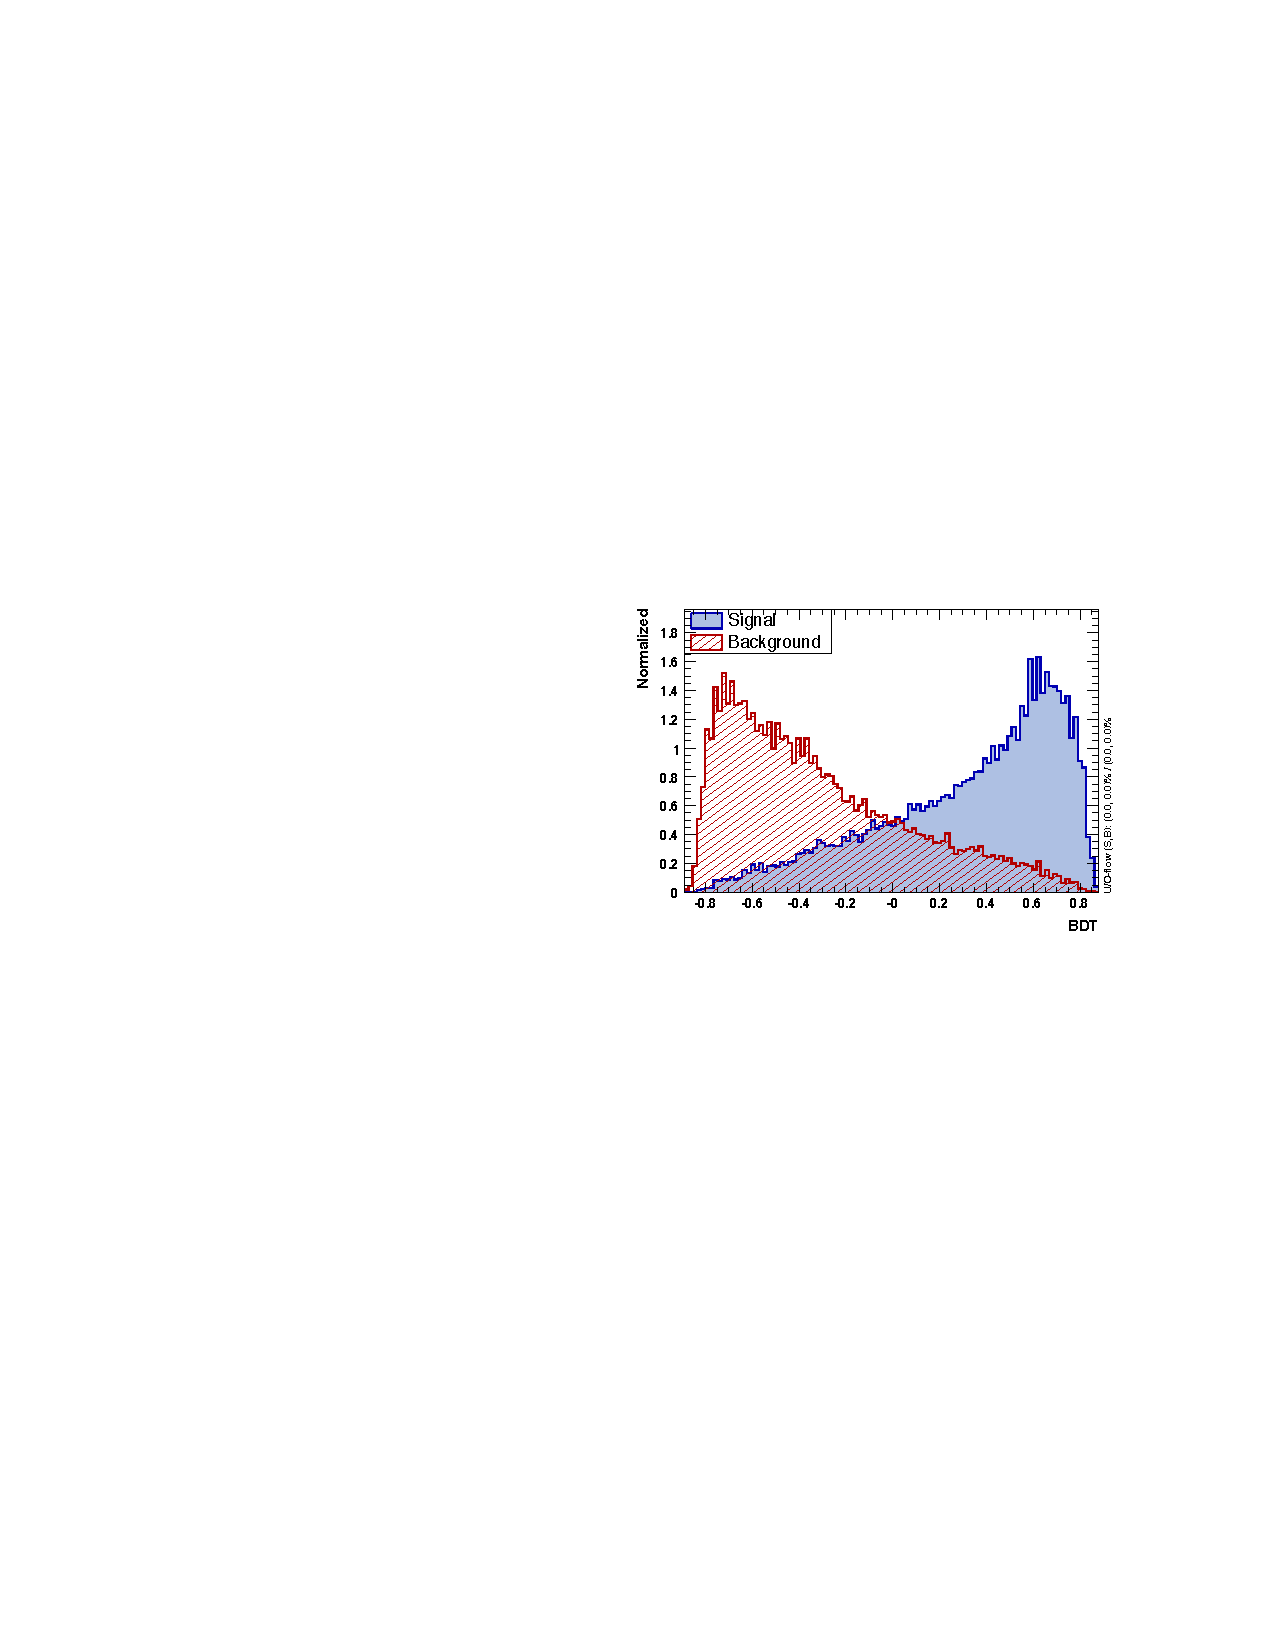
\includegraphics[height=2in]{example-TMVA-BDT.pdf}
 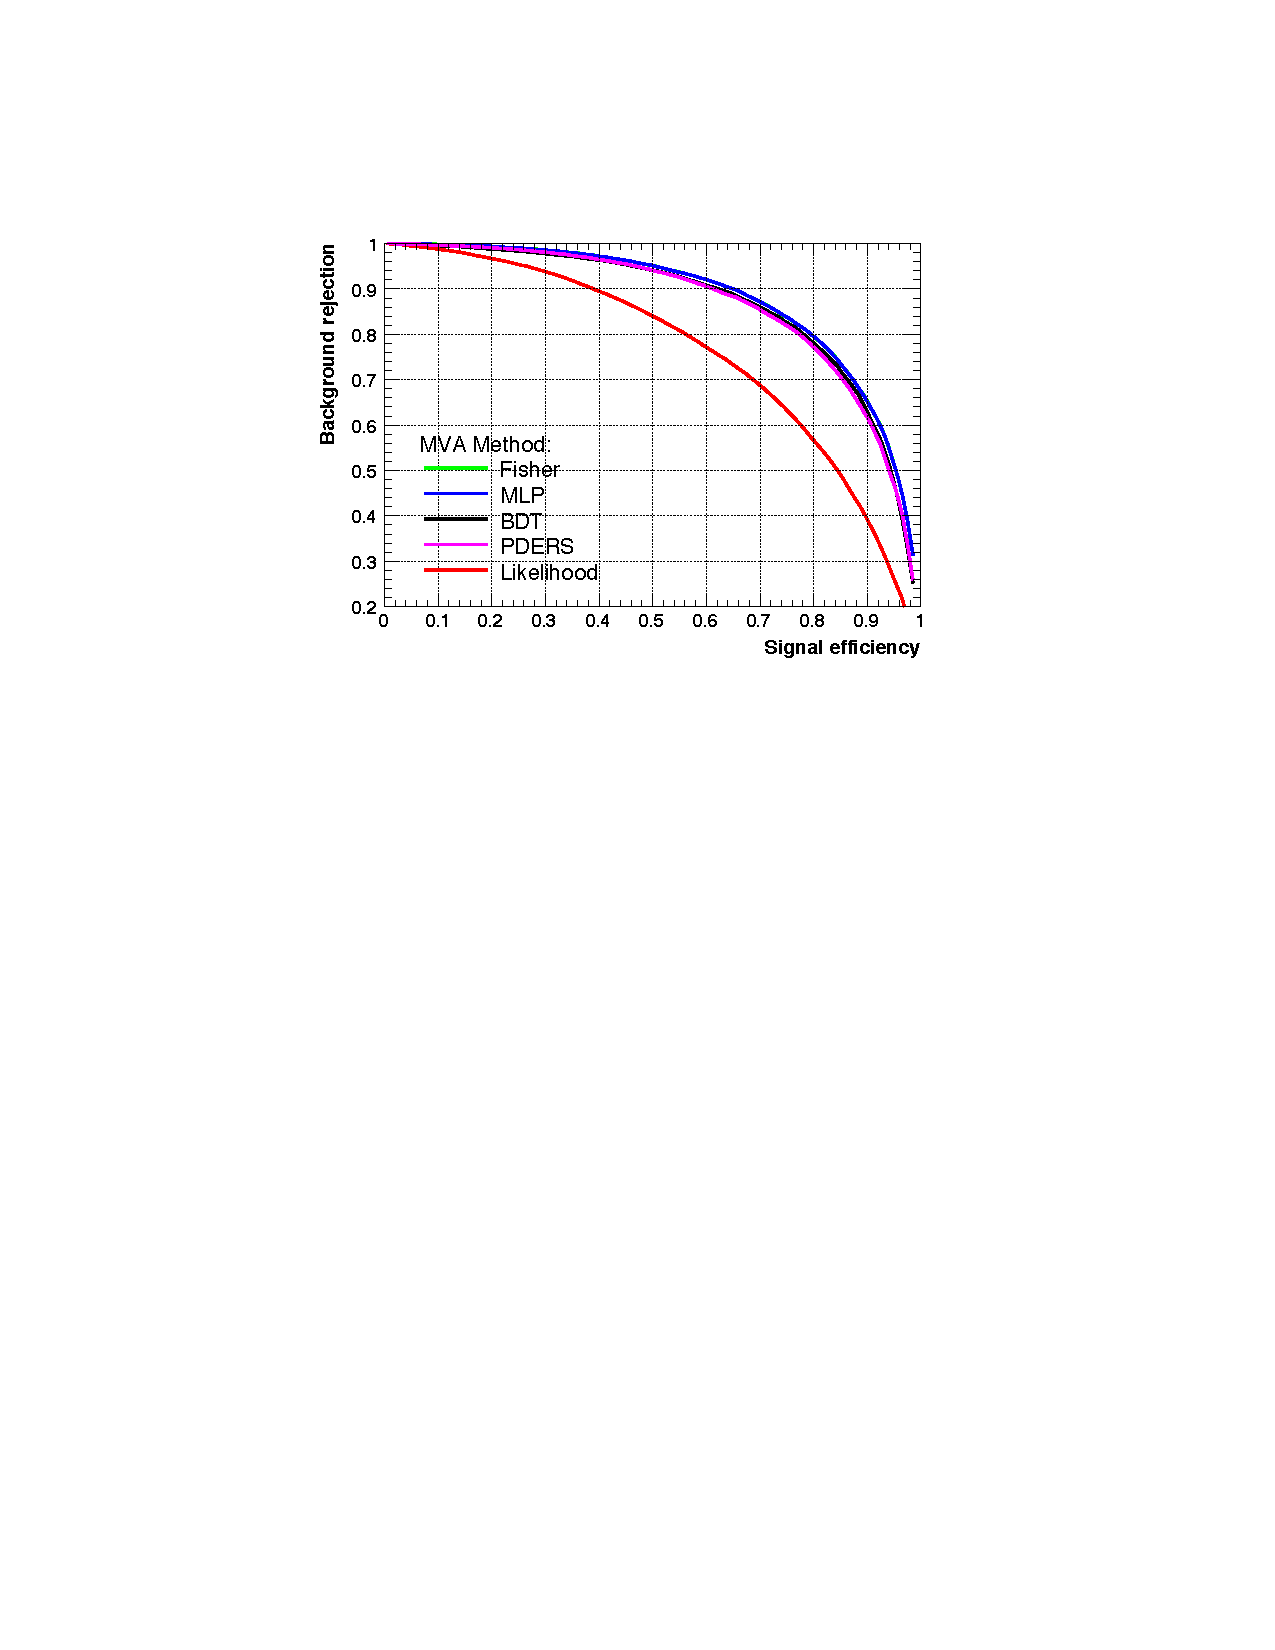
\includegraphics[height=2in]{example-TMVA-ROC.pdf}
\caption{Left: an example of the distributions $p_b(\hat s|\nu)$ and $p_s(\hat s|\nu)$ when the classifier $s$ is a boosted-decision tree (BDT). Right: the corresponding ROC curve (right) for this and other classifiers. (Figures taken from TMVA manual.)}
\label{fig:tmva}
\end{center}
\end{figure}
%\bigskip

These steps lead to a subsequent statistical analysis where one observes in data \\
${D=(x_1, \dots, x_n)}$. For each event, the classifier is evaluated and one performs inference on a parameter $\mu$ related to the presence of the signal contribution. In particular, one forms the statistical model
\begin{equation}\label{eq:typicalML}
p( D \,|\, \mu, \nu) = \prod_{e=1}^n \, \left[\, \mu p_s( \hat s(x_e) \, |\,  \nu)  + (1-\mu)\, p_b( \hat s(x_e) \,|\, \nu) \,\right] \; ,
\end{equation}
where $\mu=0$ is the null (background-only) hypothesis and $\mu>0$ is the alternate (signal-plus-background) hypothesis.\footnote{Sometimes there is an additional Poisson term when expected number of signal and background events is known, which is referred to as an extended likelihood.} Typically, we are interested in inference on $\mu$ and $\nu$ are nuisance parameters.

\subsection{Comments on typical usage of machine learning in HEP}

Nuisance parameters are an after thought in the typical usage of machine learning in HEP. In fact, most machine learning discussions would only consider $p_b(x)$ and $p_s(x)$. However, as experimentalists we know that we must account for various forms of systematic uncertainty, parametrized by nuisance parameters $\nu$. In practice, we take the classifier as fixed and then propagate uncertainty through the classifier as in Eq.~\ref{eq:typicalML}. Building the distribution $p(\hat s|\nu)$ for values of $\nu$ other than the nominal $\nu_0$ used to train the classifier can be thought of as a calibration necessary for classical statistical inference; however, this classifier is clearly not optimal for $\nu \ne \nu_0$.

\subsection{A more powerful  approach}

The standard use of machine learning in HEP can be improved by training a parametrized, discriminative classifier corresponding to the generalized likelihood ratio test 
\begin{equation}
\lambda(\mu) = \frac{p(D|\mu, \hat{\hat{\nu}})}{p(D|\hat \mu, {\hat{\nu}})} \;,
\end{equation}
following the approach outlined in Section~\ref{S:GLR}. 

There is an interesting distinction between this approach and the standard use in which the classifier is trained for a fixed $\nu_0$. In the standard use one trains a classifier for signal vs. background, which is equivalent (in an ideal setting) to training a classifier for  null (background-only) vs. alternate (signal-plus-backgound) as 
\begin{equation}
 \frac{p(x| 0, \nu_0)}{p(x|\hat \mu, \nu_0)} =  \frac{p_b(x| \nu_0)}{ \mu p_s( x_e \, |\,  \nu_0)  + (1-\mu)\, p_b( x_e \,|\, \nu_0)} = \left[ c_1 + c_2   \frac{p_s(x| \nu_0)}{ p_b( x_e \,|\, \nu_0)} \right ]^{-1} \; ,
\end{equation}
and $c_1$ and $c_2$ are constants. Specifically, the two  likelihood ratios are in one-to-one correspondence, so an ideal algorithm would lead to equivalent tests. In contrast, in the case of the generalized likelihood ratio test 
\begin{equation}
 \frac{p(x| 0, \hat{\hat{ \nu}})}{p(x|\hat \mu, \hat\nu)} =  \frac{p_b(x| \hat{\hat{ \nu}})}{ \hat \mu p_s( x_e \, |\,  \hat\nu)  + (1- \hat \mu )\, p_b( x_e \,|\, \hat \nu)} \; ,
\end{equation}
the background components don't cancel and there is an additional term $p_b(x| \hat{\hat{ \nu}})/p_b(x| {\hat{ \nu}})$.
In practice, with classifiers of finite capacity, there will be some tradeoff between taking into account this additional term and the more challenging learning problem when $\mu$ is very small. 

\subsection{Decomposing tests between mixture models into their components}

It is common that the generative model for the low-level features is a mixture model of several components
\begin{equation}
p(x|\theta)=\sum_c w_c(\theta) p_c(x| \theta) \;.
\end{equation}
In the case of particle physics, the distributions $p(x|\theta)$ is not a Gaussian Mixture Model, but mixture of  complicated distributions associated to relatively few types of particle interactions. Moreover, when searching for a new particle, the null hypothesis would correspond to some of the coefficients $w_c=0$ while the alternate ``signal-plus-background'' hypothesis would have $0<w_{c\in \rm signal} \ll w_{c\in \rm background}$. In some cases $w_{c\in \rm signal} / w_{c\in \rm background} <10^{-6}$, which means the alternate hypothesis is a small perturbation to the null hypothesis. This can be a challenge for typical classifiers because they should devote their capacity to the region where $p_{c\in \rm signal}(x) / p_{c\in \rm background}(x)$ is relatively large. Lastly, even when the distributions $p_c(x|\theta)$ are well known, it is often the case that the coefficients are uncertain or treated as completely unknown. These all present challenges to machine learning algorithms that aim to learn $s(x; \theta_0, \theta_1)$.

%\begin{equation}
%\frac{p(x|\theta_0)}{p(x|\theta_1)}= \frac{\sum_c w_c(\theta_0) p_c(x| \theta_0)}{\sum_c w_c(\theta_1) p_c(x| \theta_1)} 
%\end{equation}
%
%\begin{equation}
%\frac{p(x|\theta_0)}{p(x|\theta_1)}= \sum_c \frac{ w_c(\theta_0) p_c(x| \theta_0)}{\sum_{c'} w_{c'}(\theta_1) p_{c'}(x| \theta_1)} 
%\end{equation}

However, it is possible to re-write the target likelihood ratio between two mixture models in terms of pairwise classification problems. 
\begin{eqnarray}
\frac{p(x|\theta_0)}{p(x|\theta_1)} & =& \frac{\sum_c w_c(\theta_0) p_c(x| \theta_0)}{\sum_c w_c(\theta_1) p_c(x| \theta_1)} 
\\
%&=& \sum_c \frac{ w_c(\theta_0) p_c(x| \theta_0)}{\sum_{c'} w_{c'}(\theta_1) p_{c'}(x| \theta_1)} \\
%&=& \sum_c \left[ \frac{\sum_{c'} w_{c'}(\theta_1) p_{c'}(x| \theta_1)}{ w_c(\theta_0) p_c(x| \theta_0)}  \right]^{-1} \\
&=& \sum_c \left[ \sum_{c'} \frac{ w_{c'}(\theta_1)}{w_c(\theta_0)} \frac{ p_{c'}(x| \theta_1)}{  p_c(x| \theta_0)}  \right]^{-1} \\
&=& \sum_c \left[ \sum_{c'} \frac{ w_{c'}(\theta_1)}{w_c(\theta_0)} \frac{ p_{c'}(s_{c,c',\theta_0, \theta_1}| \theta_1)}{ p_c(s_{c,c',\theta_0, \theta_1}| \theta_0)}  \right]^{-1} 
\end{eqnarray}
The second line is a trivial, but useful decomposition into pair-wise classification between $p_{c'}(x|\theta_1)$ and $p_c(x|\theta_0)$.  The third line uses Theorem 1 to relate the high-dimensional likelihood ratio into an equivalent calibrated likelihood ratio based on the univariate density of the corresponding classifier, denoted $s_{c,c',\theta_0, \theta_1}$. In the situation where the only free parameters of the mixture model are the coefficients $w_c$, then the distributions $p_{c}(s_{c,c',\theta_0, \theta_1}| \theta)$ are independent of $\theta$ and can be pre-computed (after training the discriminative classifier, but before performing the generalized likelihood ratio test).


%
%The idea here is to combine the calibration of the distributions of the classifier output and a more optimal family of classifiers $\hat s(x; \nu_0, \nu_1)$. Creating the family of classifiers is straight forward, one simply augments the training data with $x$ examples drawn from several values of $\nu$ and then includes the corresponding value of $\nu$ as an input to the classifier. Thus $\{x_e,c_e\} \to \{x_e,\nu_{0,e},\nu_{1,e}, c_e\}$ leading to a parametrized learner $\hat s(x)\to \hat s(x;\nu_0, \nu_1)$. This leads to a complication: one does not know the value of $\nu$ to use when evaluating the parametrized classifier $\hat s(x;\nu_0, \nu_1)$, so one cannot simply pre-compute $\hat s_e$ before performing the likelihood fit.  However, when performing a likelihood ratio test, one can calculate the maximum likelihood estimate and conditional maximum likelihood estimate according to Eq.~\ref{eq:mle} and then form the equivalent likelihood ratio test according to Eq.~\ref{eq:equivLRtest}. 


%Equivalently, once one has determined $\hat{\theta}$ and $\hat{\hat{\theta}}$, then one can specify the parameters of the mapping $s(x;\hat{\hat{\theta}}, \hat{\theta})$ and then following Eq.~\ref{eq:NP} form the likelihood
%\begin{equation}\label{eq:parametrizedML}
%p( D \,|\, \mu, \nu) = \prod_{e=1}^n \, \left[\, \mu p_s( s(x_e;\nu_0, \nu_1) \, |\,  \nu)  + (1-\mu)\, p_b( s(x_e;\nu_0, \nu_1) \,|\, \nu) \,\right] \; ,
%\end{equation}
%which is a natural generalization of Eq.~\ref{eq:typicalML}.

%The construction in Eq.~\ref{eq:parametrizedML} presents a computational challenge as for each value of $\nu$ one has a new mapping $s: x\to\mathbb{R}$. The most naive realization of this would be to generate synthetic data $\{x_e\}$ according to $p_c(x|\nu)$, evaluate $s(x_e ; \nu_0, \nu_1)$, and then use a histogram, kernel density, or other non-parametric density estimation procedure to estimate $p_c( s | \nu)$. This approach is not realistic in situations where $p_c(x|\nu)$ is realized with expensive computer simulations; thus, some interpolation strategy or emulator over a fixed set of parameter points $\{\nu_i\}$ would typically be used.

\subsection{Related work}

%Refs to include:
%\cite{ClaytonScott,AndrewY.Ng,SamT.Roweis,EricP.Xing,SujaySanghavi,BiancaZadrozny,Zadrozny2001,}

\cite{ClaytonScott} and \cite{JMLR:v14:tong13a} consider the machine learning problem associated to Neyman-Pearson hypothesis testing. As in this work, they consider the situation where one does not have access to the underlying distributions, but only has i.i.d. samples from each hypothesis. This work generalizes that goal from the Neyman-Pearson setting to generalized likelihood ratio tests and emphasizes the connection with classification. Perhaps a  formal treatment similar to the Neyman-Pearson case can be brought to bear in this more general setting.
\cite{TommiJaakkola} explore a way of leveraging generative models to derive kernel functions for use in discriminative methods. This interesting work is distinct from the point made here in which the generative model is being used for the purpose of providing training data and calibration.  \cite{McCallum}
 consider a hybrid generative/discriminative classifier; however, the goal of that work is not to leverage a generative model for the data, but to use both approaches to learn different subsets of the parameters in a single hybrid classifier.  \cite{BiancaZadrozny} emphasize the importance of calibrated probability estimates from decision trees and naive Bayesian classifiers and investigate various approaches to achieve this. In contrast to that work, we are not interested in calibrated probability estimates for $p(y|x)$ for individual events, but instead we use the calibration to correct for non-linear transformations of the target likelihood ratio and, perhaps, to provide calibrated p-values based on those likelihood ratio tests. \cite{Ihler2004} take on a different problem (tests of statistical independence) by using machine learning algorithms to find  scalar maps from the high-dimensional feature space that achieve the desired statistical goal when the fundamental high-dimensional test is intractable.


\section{Conclusions}

We have shown that a parametrized family of discriminative classifiers $s(x; \theta_0, \theta_1)$ trained and calibrated with a generative model $p(x|\theta)$ can be used to approximate statistical inference likelihoodased on the  ratio $p(x|\theta_0)/p(x|\theta_1)$ when it is not possible to evaluate the densities $p(x|\theta)$ for an arbitrary $x$. This approach leverages the power of machine learning in a classical statistical setting.

%\section{Possible Extensions}
%The approach describe thus far has been agnostic as to the type of classifier used to produce $s(x)$ and $s(x; \nu)$. In practice, we have used standard packages for the training of these learners. In particular, the loss function for these learning algorithms is based on classification performance of individual $(x_e, c_e)$ feature $\to$ target examples. However, in overarching statistical procedure that uses the statistical model in Eq.~\ref{eq:typicalML} or \ref{eq:parametrizedML} the quantity we wish to optimize is a property of an entire dataset $\{x_e\}$ or ensembles of datasets that can be generated from the statistical models $p_c(x|\theta)$. 
%
%For example, in typical hypothesis testing problems posed in the Neyman-Pearson context one would be interested in minimizing type II error under a fixed rate of typeI error rate. In the presence of systematic uncertainty and nuisance parameters, the loss function may become more complicated. The recent Higgs boson machine learning challenge hosted by Kaggle, the evaluation was the approximate median significance (AMS) that characterized the power of a hypothesis test between $\mu=0$ (the background only hypothesis) and $\mu=\mu_0$ (the signal+background hypothesis, where $\mu_0$ is a small number reflecting the small Higgs signal that would be found in addition to the much larger background process) in the presence of uncertainty on the background normalization. 
%Interestingly, the top entries to the challenge did not improve by focusing on this alternative loss function 
%in training their classifier, but instead used it for the optimization of a threshold on the score (a working point on the ROC curve) that was related to the way the challenge was designed. This suggests that the standard 
%classification loss functions lead to similar optimizations and that refinements for the custom loss functions
%are not easy to come by.
%
%More generally, there is an avenue of research associated to custom loss functions specifically designed 
%for these real world statistical problems. One direction might be to choose loss functions that make 
%some balance between the standard classification loss, take into account robustness with respect to nuisance parameters, and population-level quantities like type I and II error.
%
%\subsection{A different starting point}
%
%Instead of evolving from the traditional usage of ML in HEP, let's start from scratch with $p_c(x|\theta)$ and a well defined objective.  
%
%\subsubsection{Simple Hypothesis Testing}
%
%Consider the situation of simple hypothesis testing between the background-only $\mu=0$ and signal+background hypothesis $\mu=\mu_0=\nu_s/(\nu_s+\nu_b)$ for $\theta=\theta_0$.  Let us assume that not only can we use the $p_c(x|\theta_0)$ as a generative model, but that we can evaluate the probability density at any point $x$.  The statistical model is given by
%\begin{equation}\label{eq:NP}
%p( D \,|\, \mu, \theta) = \prod_{e=1}^n \, \left[\, \mu p_1( x_e \, |\,  \theta)  + (1-\mu)\, p_b( x_e \,|\, \theta) \,\right] \; .
%\end{equation}
%The objective is to find a  test statistic $T(D)$ (a map from the space of the data to $\mathbb{R}$)  
%and a threshold $k_\alpha$ that minimizes the rate of type-II error (i.e. $P(T(D) < k_\alpha | \mu=\mu_0, \theta_0) = \beta$ under the constraint of a fixed rate of type-I error ( i.e.  $P(T(D) > k_\alpha | \mu=0, \theta_0) = \alpha$ ).
%The Neyman-Pearson lemma states that the optimal test statistic is the likelihood ratio, or equivalently, the log-likelihood ratio 
%\begin{equation}
%T =  \log \frac{p(D | \mu=\mu_0, \theta_0)}{p(D | \mu=0, \theta_0)}
%\end{equation}
%When the $x_e$ are i.i.d., then the log-likelihood ratio expands into a sum
%\begin{equation}
%T =   \sum_{e=1}^n \underbrace{\log \left[ 1+c_1\frac {p_1(x_e | \theta_0) }{ p_b(x_e | \theta_0) } \right]}_{q(x_e)} + c_2\;,
%\end{equation}
%where $c_1=\mu/(1-\mu)$ and $c_2=\lop(1-\mu)$ are constants for the simple hypothesis test.
%
%Here we see that the optimal $T$ for the experiment is composed of a sum over events of a linear linear function of the per-event function $q(x)$. A monotonic, but non-linear function of $q(x)$ would not lead to an equivalent hypothesis test. 
%
%The important part of the per-event function $q(x)$ is that it defines contours in the feature space $x$. These contours are also equivalent to the function $p_1(x|\theta_0)/p_b(x|\theta_0)$, the signal-to-background ratio. If we can find a machine learner $s(x)$ that is a monotonic function of $p_1(x|\theta_0)/p_b(x|\theta_0)$ it will share the same contours. Then the remaining challenge is to find the appropriate rescaling that gives back  linear function $q(x)$. 
%
%\textbf{Postulate:}
%\begin{equation}
%T' = \sum_{e=1}^n \underbrace{\log \left[ 1+c_1\frac {p_1(s(x_e) | \theta_0) }{ p_b(s(x_e) | \theta_0) } \right]}_{q(s_e)} \;,
%\end{equation}
%leads to an equivalent test, where $s_e \equiv s(x_e)$
%\begin{equation}
%p_c(s) = \int dx \, \delta(s-s(x)) \, p_c(x)  \,  |\partial s / \partial x|^{-1}
%\end{equation}
%
%
%
%Note, in order to form the hypothesis test, one still needs to build the build the $p_0(T|\theta)$ to calibrate the threshold  $T>k_\alpha$ that gives rise to a test of size $\alpha$. 
%
%
%
%\textbf{Proof (in progress):}
%
%We want to show density is the same 
%
%\begin{equation}
%p_c(q_x) = \int dx \delta(q_x-q_x(x)) p_c(x) / |\partial q_x / \partial x|
%\end{equation}
%
%\begin{equation}
%p_c(q_s) = \int dx \delta(q_s-q_s(s(x))) \, p_c(x) \, / |\partial q_s / \partial x|
%\end{equation}
%sufficient to show $q(x_e) = q(s(x_e))$.  Here we use that $p_1(x)/p_0(x)=\textrm{const}$ for all points on the level-set $\Omega_c$ given by $ \delta(c-s(x))$. 
%\begin{equation}
%\frac {p_1(c | \theta_0) }{ p_0(c | \theta_0) } = 
%\frac { \int dx \delta(c-s(x)) \, p_1(x_e | \theta_0) }{ \int dx \delta(c-s(x)) \, p_0(x | \theta_0)  } = 
%\frac {c \int dx \delta(c-s(x)) \, p_0(x | \theta_0)  }{ \int dx \delta(s-s(x)) \, p_0(x | \theta_0)  } = c =\frac {p_1(x | \theta_0) }{ p_0(x | \theta_0) } 
%\end{equation}
%
%
%
%%\begin{equation}
%%p_c(q_s) = \int ds \delta(q_s-q_s(s)) \,p_c(s) \, / |\partial q_s / \partial s|
%%\end{equation}
%
%
%This is the test statistic that one would naturally get from constructing the likelihood function for the 1-d distributions of the output of the machine learner
%\begin{equation}\label{eq:NP}
%p( \{s_e\} \,|\, \mu, \theta) = \prod_{e=1}^n \, \left[\, \mu p_1( s_e \, |\,  \theta)  + (1-\mu)\, p_0( s_e \,|\, \theta) \,\right] \; .
%\end{equation}
%Thus this motivates Eq.~\ref{eq:typicalML} in the more general case. 
%
%
%Question:
%Where does this fit in:
%\begin{equation}
%T'' = \sum_{e=1}^n \underbrace{ \log \left[ 1+c_1 s(x_e) \right] }_{q'(s_e)} \;,
%\end{equation}
%
%
%
%Usefulness:
%If we can readily compute $p_c(x|\theta_0)$, then there would be no need for machine learning algorithms. However,  these densities are often difficult to compute though one can readily use them as a generative model to produce samples. In that case, one might wish to use a machine learning algorithm to find $s(x) \approx p_1(x|\theta_0) / p_0(x|\theta_0)$. 
%
%Conclusion, while it is possible to start directly with the Neyman-Pearson loss function of type-II error under the constraint of fixed size and try to find a per-experiment learner $T(D)$, it is more convenient to cast the problem in terms of learning a per-event function $s(x)$, and then calibrate it to be a linear function of $q(x)$.
%
%\newpage
%
%Given $x\in \mathbb{R}^n$ and two smooth, real-valued functions $p_1(x)$ and $p_0(x)$ define 
%\begin{equation} 
%s(x)=\frac{p_1(x)}{p_2(x)}
%\end{equation}.
%Define $p_1(c) = \int dx \delta(c - s(x) ) \, p_1(x)$ and $p_0(c) = \int dx \delta(c - s(x) ) \, p_0(x)$.
%I wish to show
%\begin{equation}
%\frac{p_1(c)}{p_0(c)} = \frac{p_1(x)}{p_0(x)}
%\end{equation}
%$\forall x \ni s(x)=c$.
%
%Sketch of Proof: 
%let $\Omega_{c}$ be the level set $\{x \mid s(x) = c \}$ and $\hat{n}=\nabla s(x) / |\nabla s(x)|$ be the perpendicular direction to the surface at the point $x$. The  coordinate perpendicular to $\Omega$ can be written $y = x+\epsilon \hat{n}$. In these coordinates, the integral $\int dx \to \int d\Omega d\epsilon$, thus
%\begin{equation}
%p_1(c) = \int dx \delta(c-s(x)) p_1(x) = \int d\Omega p_1(x) / |\partial s(x)/\partial \epsilon|
%\end{equation}
%Similarly for $p_0(c)$. We can factor out of the integral $s(x)=p_1(x)/p_0(x)$ since it is constant over $\Omega$.
%Thus
%\begin{equation}
%p_1(c) = \int dx \delta(c-s(x)) p_1(x) = \int d\Omega p_1(x) / |\partial s(x)/\partial \epsilon| = s(x) \int d\Omega p_0(x) / |\partial s(x)/\partial \epsilon|
%\end{equation}
%and we arrive at the result
%\begin{equation}
%\frac{p_1(c)}{p_0(c)} = \frac{s(x) \int d\Omega p_0(x) / |\partial s(x)/\partial \epsilon|}{ \int d\Omega p_0(x) / |\partial s(x)/\partial \epsilon|} = \frac{p_1(x)}{p_0(x)} \;.
%\end{equation}
%
%
%
%
%\subsection{misc notes}
%
%
%
%
%The distribution of $s$ is fully determined by the mapping $s(x_e; \theta_0, \theta_1)$ and the distribution $p(x)$, which we can write
%\begin{equation}
%p(s_e) = \int dx \, \delta(s_e-s(x)) \, p(x)  \; .
%\end{equation}
%\textbf{NEED Jacobian for x $\to$ s independent of delta function part, or double counting?}
%
%
%\textbf{Theorem 1:}
%Let $\Omega_{c}$ be the level set $\{x \mid s(x) = c \}$ and $\hat{n}=\nabla s(x) / |\nabla s(x)|$ be the orthonormal vector to the surface at the point $x$. The component perpendicular to $\Omega_c$ can be written $x+\epsilon \hat{n}$. In these coordinates, we rewrite integral $\int dx \to \int d\Omega_c d\epsilon$, thus
%\begin{equation}
%p_1(c) = \int dx \delta(c-s(x)) p_1(x) = \int d\Omega_c p_1(x)  / | \hat{n} \cdot \nabla q_s  |
%\end{equation}
%Similarly for $p_0(c)$. We can factor out of the integral $s(x)=p_1(x)/p_0(x)$ since it is constant over $\Omega_c$.
%Thus
%\begin{equation}
%p_1(c) = \int dx \delta(c-s(x)) p_1(x) = \int d\Omega p_1(x) / |\partial s(x)/\partial \epsilon| = s(x) \int d\Omega p_0(x)  / | \hat{n} \cdot \nabla q_s  |
%\end{equation}
%and we arrive at the result
%\begin{equation}
%\frac{p_1(c)}{p_0(c)} = \frac{s(x) \int d\Omega p_0(x) / |\partial s(x)/\partial \epsilon|}{ \int d\Omega p_0(x) / |\partial s(x)/\partial \epsilon|} = \frac{p_1(x)}{p_0(x)} \;\hspace{3em} \forall x\in\Omega_c.
%\end{equation}
%
%
%
%
%
%Define $p_1(c) = \int dx \delta(c - s(x) ) \, p_1(x)$ and $p_0(c) = \int dx \delta(c - s(x) ) \, p_0(x)$.
%I wish to show
%\begin{equation}
%\frac{p_1(c)}{p_0(c)} = \frac{p_1(x)}{p_0(x)}
%\end{equation}
%$\forall x \ni s(x)=c$.
%
%
%Given $x\in \mathbb{R}^n$ and two smooth, real-valued functions $p_1(x)$ and $p_0(x)$ define 
%\begin{equation} 
%s(x)=\frac{p_1(x)}{p_0(x)}
%\end{equation}.
%Define $p_1(c) = \int dx \delta(c - s(x) ) \, p_1(x)$ and $p_0(c) = \int dx \delta(c - s(x) ) \, p_0(x)$.
%I wish to show
%\begin{equation}
%\frac{p_1(c)}{p_0(c)} = \frac{p_1(x)}{p_0(x)}
%\end{equation}
%$\forall x \ni s(x)=c$.
%
%Sketch of Proof: 
%let $\Omega_{c}$ be the level set $\{x \mid s(x) = c \}$ and $\hat{n}=\nabla s(x) / |\nabla s(x)|$ be the perpendicular direction to the surface at the point $x$. The  coordinate perpendicular to $\Omega$ can be written $y = x+\epsilon \hat{n}$. In these coordinates, the integral $\int dx \to \int d\Omega d\epsilon$, thus
%\begin{equation}
%p_1(c) = \int dx \delta(c-s(x)) p_1(x) = \int d\Omega p_1(x) / |\partial s(x)/\partial \epsilon|
%\end{equation}
%Similarly for $p_0(c)$. We can factor out of the integral $s(x)=p_1(x)/p_0(x)$ since it is constant over $\Omega$.
%Thus
%\begin{equation}
%p_1(c) = \int dx \delta(c-s(x)) p_1(x) = \int d\Omega p_1(x) / |\partial s(x)/\partial \epsilon| = s(x) \int d\Omega p_0(x) / |\partial s(x)/\partial \epsilon|
%\end{equation}
%and we arrive at the result
%\begin{equation}
%\frac{p_1(c)}{p_0(c)} = \frac{s(x) \int d\Omega p_0(x) / |\partial s(x)/\partial \epsilon|}{ \int d\Omega p_0(x) / |\partial s(x)/\partial \epsilon|} = \frac{p_1(x)}{p_0(x)} \;.
%\end{equation}
%
%
%
%
%
%
%
%Note, in order to form the hypothesis test, one still needs to build the build the $p_0(T|\theta)$ to calibrate the threshold  $T>k_\alpha$ that gives rise to a test of size $\alpha$. 
%
%
%
%\textbf{Proof (in progress):}
%
%We want to show density is the same 
%
%\begin{equation}
%p(q_x|\theta) = \int dx \delta(q_x-q_x(x)) p(x|\theta)  / | \hat{n} \cdot \nabla q_s  |
%\end{equation}
%
%\begin{equation}
%p(q_s|\theta) = \int dx \delta(q_s-q_s(s(x))) \, p(x|\theta) \, / | \hat{n} \cdot \nabla q_s  |
%\end{equation}
%sufficient to show $q(x_e) = q(s(x_e))$.  Here we use that $p_1(x)/p_0(x)=\textrm{const}$ for all points on the level-set $\Omega_c$ given by $ \delta(c-s(x))$. 
%\begin{equation}
%\frac {p_1(c | \theta_0) }{ p_0(c | \theta_0) } = 
%\frac { \int dx \delta(c-s(x)) \, p_1(x_e | \theta_0) }{ \int dx \delta(c-s(x)) \, p_0(x | \theta_0)  } = 
%\frac {c \int dx \delta(c-s(x)) \, p_0(x | \theta_0)  }{ \int dx \delta(s-s(x)) \, p_0(x | \theta_0)  } = c =\frac {p_1(x | \theta_0) }{ p_0(x | \theta_0) } 
%\end{equation}
%
%
%
%%\begin{equation}
%%p_c(q_s) = \int ds \delta(q_s-q_s(s)) \,p_c(s) \, / |\partial q_s / \partial s|
%%\end{equation}
%
%



\section*{Acknowldgements}
KC would like to thank  
Daniel Whiteson for discussions and encouragement throughout the project, 
Alex Ihler for challenging discussions that 
led to a reformulation of the initial idea, and Shimon Whiteson for patient feedback in that process. 
KC would also like to thank Yann LeCun, Philip Stark, and Pierre Baldi for their feedback on the
project early in its conception, Bal\'azs K\'egl for discussions about the Kaggle challenge and feedback to the draft, 
and Yuri Shirman for reassuring cross checks of the Theorem.
KC is supported by the US National Science Foundation grants PHY-0854724 and PHY-0955626. 
KC is grateful to UC-Irvine for their hospitality while this research was carried out and the 
Moore and Sloan foundations for their generous support of the data science environment at NYU.

\bibliographystyle{natbib}
\bibliography{learning.bib}
%\begin{thebibliography}
%\parametrized-learning}
%\end{thebibliography

\end{document} 
